\documentclass[9pt]{beamer}
%\usetheme{CambridgeUS}
\usetheme{Antibes}
\usecolortheme[RGB={120,130,235}]{structure}

\usepackage{graphics}
\usepackage{marvosym}
\usepackage{graphicx}
\usepackage{latexsym}
\usepackage{multimedia}
\usepackage{subcaption}
\usepackage{hyperref}
\usepackage{breqn}
\newtheorem{prop}{Proposition}

%Define New Macros
%\input macros
\renewcommand\o{\omega}
\newcommand{\deriv}{\mbox{d}}
\newcommand{\Real}{\mathbb R}
\newcommand{\T}{\mathbb T}
\newcommand{\norm}[1]{\|#1\|}
\newcommand{\abs}[1]{\left\vert#1\right\vert}
\newcommand{\set}[1]{\left\{#1\right\}}
\newcommand{\subheading}[1]{\noindent \textbf{#1}}
\newcommand{\grad}{\nabla}
\newcommand{\diverg}{\textup{div} }
\newcommand{\jump}[1]{[#1]}
\newcommand{\limit}[2]{\lim_{#1 \rightarrow #2}}
\newcommand{\mollify}[1]{ \mathcal{J}_\epsilon #1 }
\newcommand{\conv}[2]{#1 \ast #2}
\newcommand{\D}{D}
\newcommand{\K}{\mathcal{K}}
\newcommand{\ineqtext}[1]{ ^{\text{\tiny #1}}}
\newcommand{\wknorm}[2]{\norm{#1}_{L^{#2,\infty}}}
%\newcommand{\wknorm}[2]{\abs{#1}_{L_w^{#2}}}
\newcommand{\wkspace}[1]{L^{#1,\infty}}
%\newcommand{\wkspace}[1]{L_w^{#1}}
\newcommand{\F}{\mathcal{F}}
\newcommand{\G}{\mathcal{G}}

%Nancy's macros
\newcommand{\reg}[1]{#1^\epsilon}
\newcommand{\Lpr}[1]{L^{#1}(\mathbb{R}^n)}
\newcommand{\Lp}[1]{L^{#1}(\Omega)}
\newcommand{\intreal}{\int_{\mathbb{R}^2}\hspace{-8pt}}
\newcommand{\energy}{\mathcal{F}}
\newcommand{\modenergy}{\mathcal{E}_H}
\newcommand{\kernel}{\mathcal{K}}
\newcommand{\into}{\int_{D}}
\newcommand{\intot}{\int_{D_T}}
\newcommand{\ball}{B_n}
\newcommand{\balltime}{B_n\times [0,T]}

\newcommand{\brak}[1]{\langle #1 \rangle} 


\DeclareMathOperator{\R}{\mathbb{R}}

\title[Personal Presentation]{Personal Presentation} 
\author[Personal Presentation]{Gareth Johnson \\[.3cm] Faculty Adviser: Prof. Ricardo Nochetto } 
\institute[] 
{
	University of Maryland\\ 
	AMSC 663: Advanced Scientific Computing I\\ 
	Supported by Johns Hopkins University Applied Physics Lab
}
\date[August 2018]{August 30, 2018}


\begin{document}
\begin{frame}
	\titlepage
\end{frame}
\section{Background}
\begin{frame}
	\begin{itemize}
		\item Born outside London, England.
		
		\item B.S. in Mathematics and Computer Science from North Carolina State University in 2017.
		
		\item Interned at IBM.
		
		\item 2nd year AMSC graduate student in the Scientific Computation track.
		
		\item Recently became a full staff member at Johns Hopkins University Applied Physics Lab. 
	\end{itemize}
	\begin{columns}
		\begin{column}{2.5cm}
			\begin{figure}
				
\includegraphics[scale=0.04]{NCSU.png}
			\end{figure}
		\end{column}
		\begin{column}{4cm}
			\begin{figure}
				
\includegraphics[scale=0.14]{jhuapl-logo.png}
			\end{figure}
		\end{column}
	\end{columns} 
\end{frame}

\section{Research Interests}
\begin{frame}{Previous Projects}
	\begin{itemize}
		\item Undergraduate Research: Worked under Pierre Gremaud on modeling blood flow. Aimed to provide appropriate BC for the circulatory system lying outside a region of interest.
		
		\item REU at UMD: Worked under Jacob Bedrossian on Numerical PDEs. Studied fluid mixing and plasma mechanics. Specifically, we studied the following equations:
		$$
			\partial_t f + \textbf{v}\cdot \grad f = \kappa \Delta f, \quad\quad 
			\partial_t p + v\cdot \grad_x p + \frac{q}{m}\big(\overrightarrow{E} + v\times \overrightarrow{B}\big)\cdot \grad_v p = C[p].
		$$
	\end{itemize}
	\begin{columns}
		\begin{column}{2cm}
			\begin{figure}
				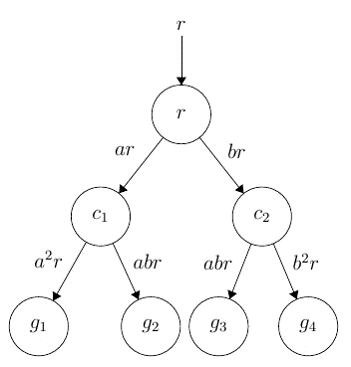
\includegraphics[scale=0.375]{Tree.png}
			\end{figure}
		\end{column}
		\begin{column}{7cm}
			\begin{figure}
					\centering
					\movie[autostart, showcontrols=true, width=.4\textwidth, externalviewer]{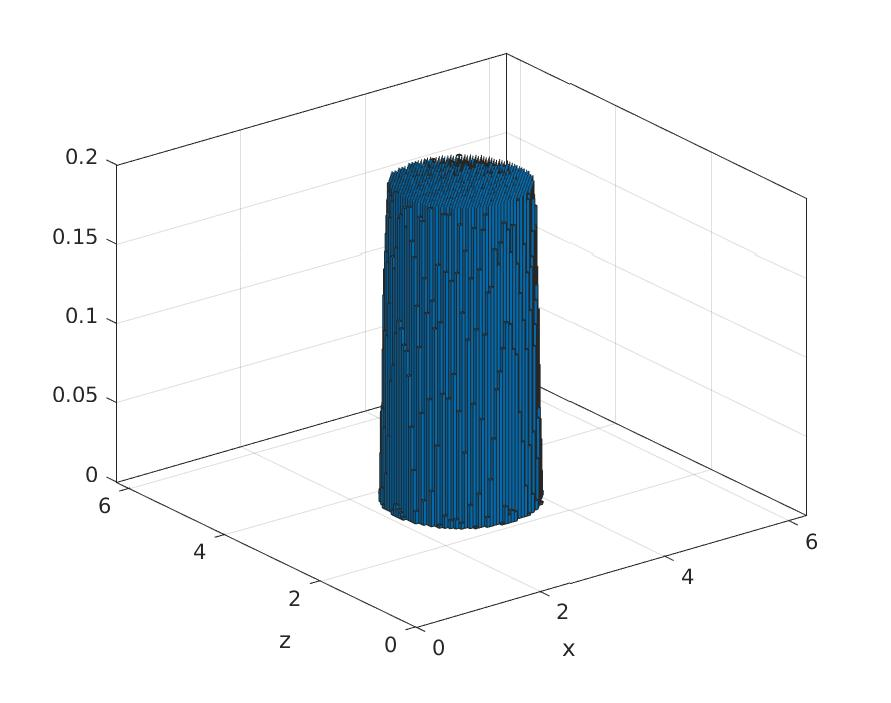
\includegraphics[scale=.15]{K=1D.jpg}}{K=1D.avi}
			\end{figure}
		\end{column}
	\end{columns} 
\end{frame}

\begin{frame}{Current Interests}
	\textbf{Academic Interests:}
	\begin{itemize}
		\item Numerical PDEs
		
		\item Mathematical Modeling, such as fluid mechanics and plasma physics.
		
		\item Computational Physics
		
		\item Numerical Analysis
	\end{itemize}
	\vspace{1cm}
	\begin{columns}
		\begin{column}{8cm}
			\textbf{Professional Interests:}
			\begin{itemize}
				\item High performance computing focusing on GPUs.
				
				\item Algorithm development for engineering problems.
				
				\item Underwater Acoustics with applications to sonar.
			\end{itemize}
		\end{column}
		\begin{column}{2cm}
			\centering
			\begin{figure}
				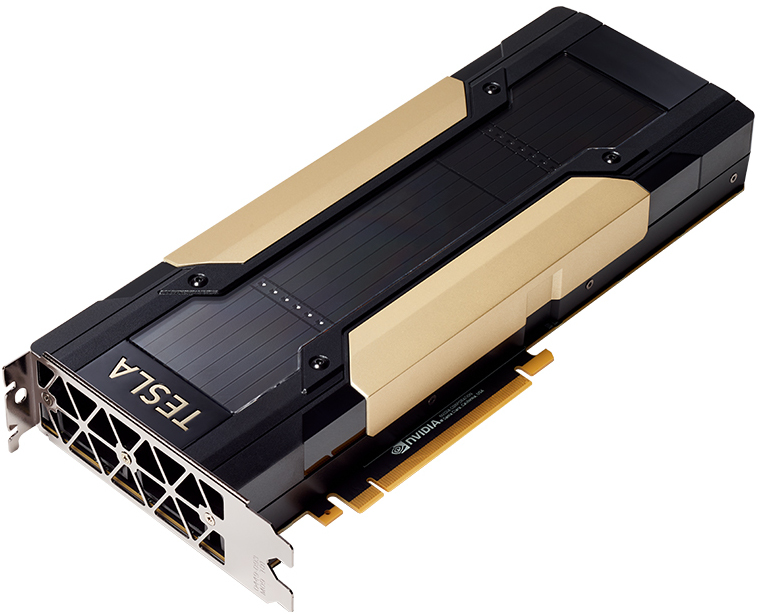
\includegraphics[scale=0.1]{v100.jpg}
			\end{figure}
		\end{column}
	\end{columns}
	
\end{frame}

\section{Personal Interests}
\begin{frame}
	\begin{itemize}
		\item Avid technology and game enthusiast. 
		
		\item Novice guitar player.
		
		\item Long distance runner.
		
		\item Currently trying to teach my cat party tricks.
	\end{itemize}
	\begin{columns}
	\begin{column}{2.5cm}
		\begin{figure}
			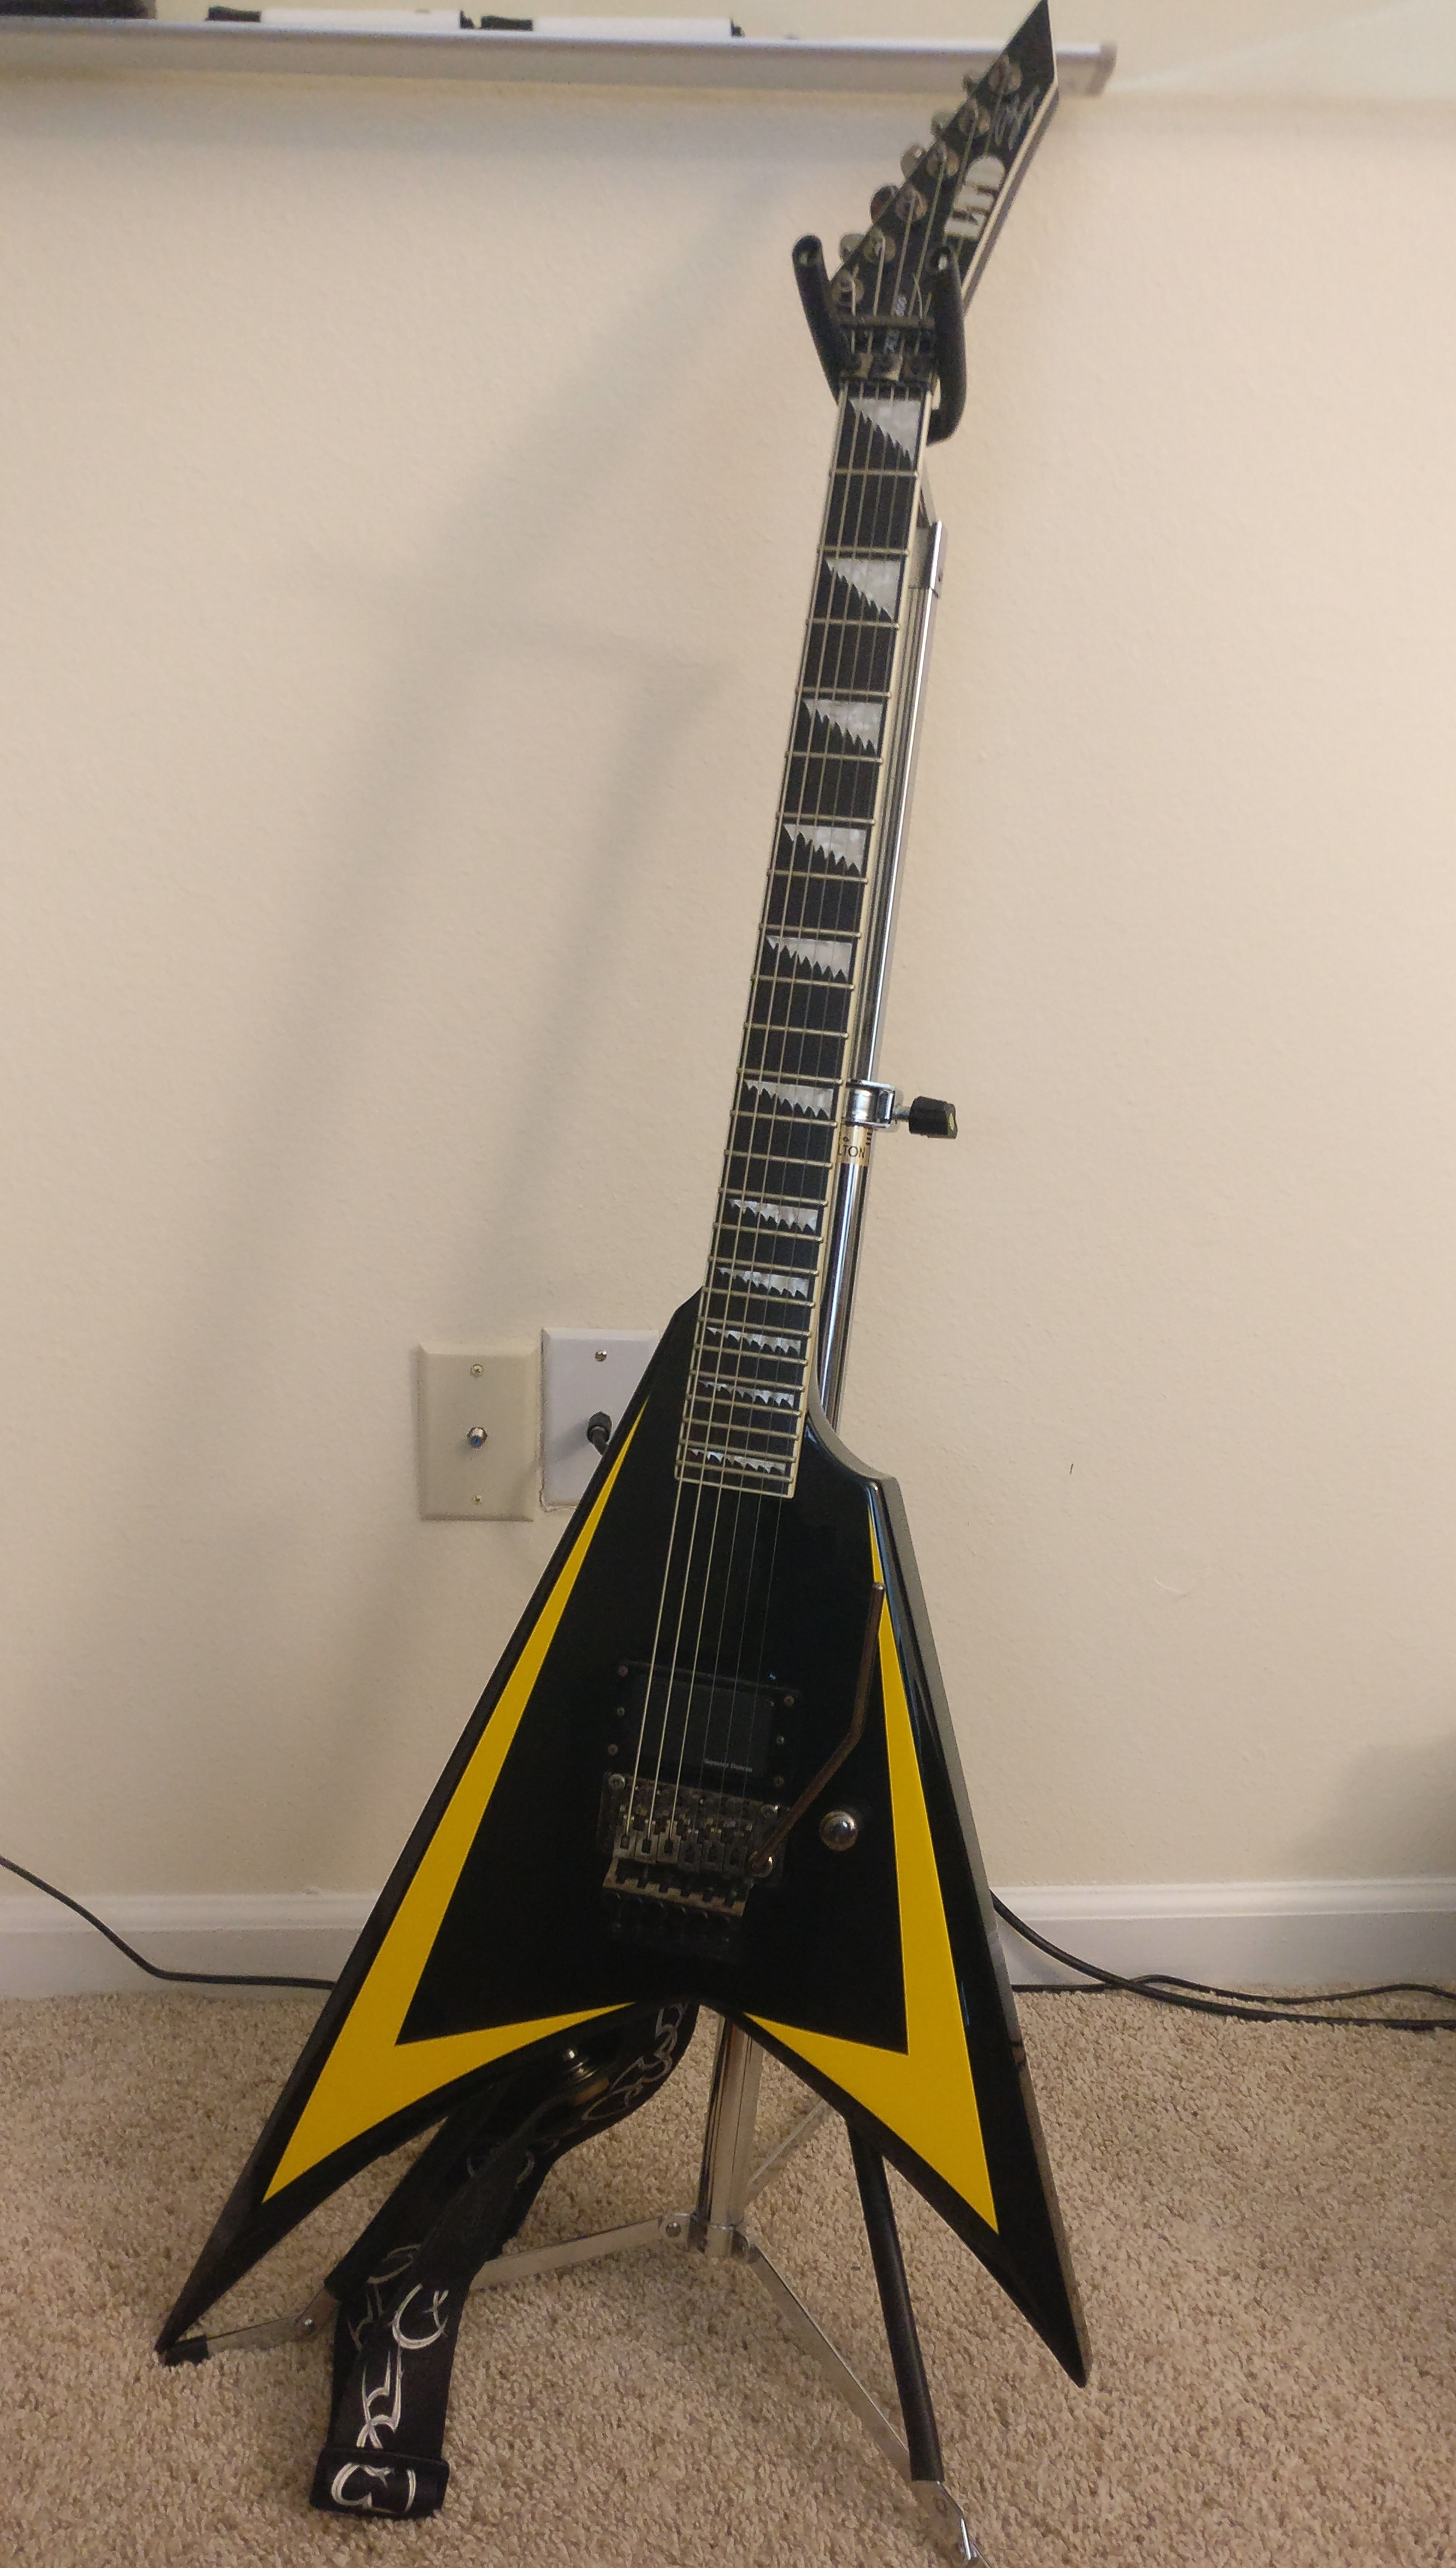
\includegraphics[scale=0.04]{guitar.jpg}
		\end{figure}
	\end{column}
	\begin{column}{4cm}
		\begin{figure}
			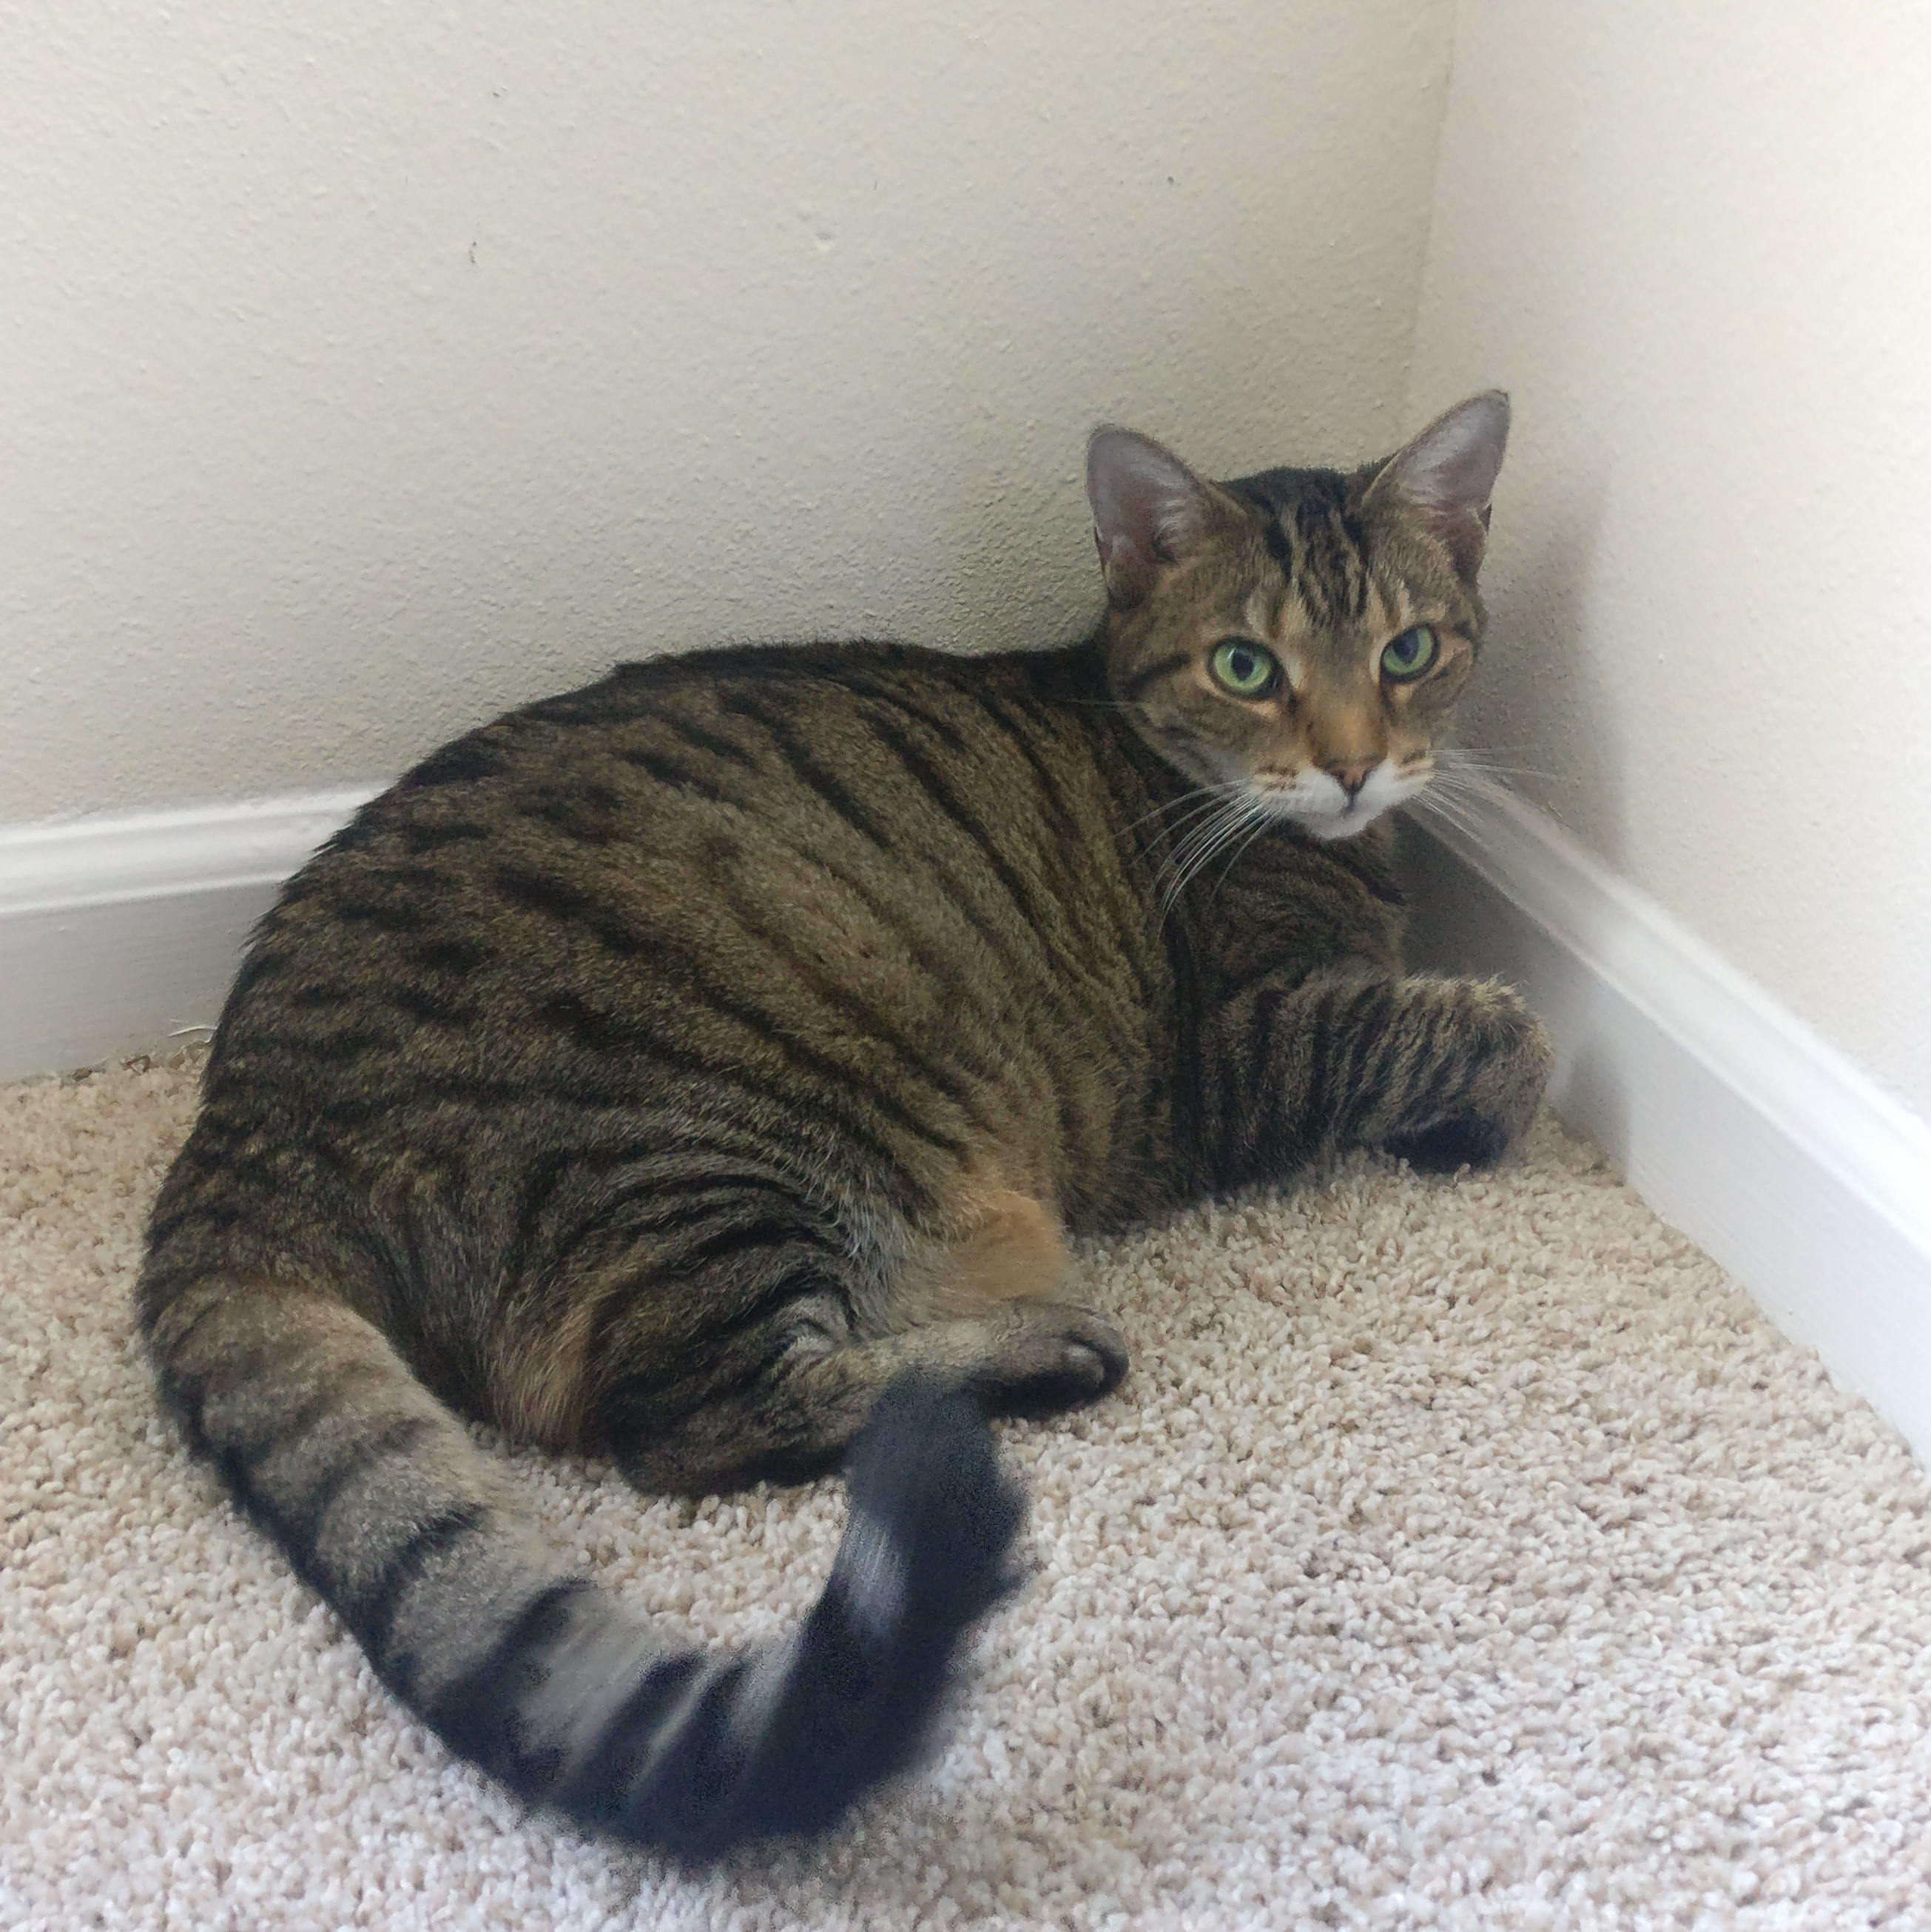
\includegraphics[scale=0.05]{boba.jpg}
		\end{figure}
	\end{column}
\end{columns} 
\end{frame}

\section{Goals for 663}
\begin{frame}
	\begin{itemize}
		\item Fulfill a degree requirement!
		
		\item Apply the Finite Element Method to a non--toy problem.
			\begin{columns}
			\begin{column}{.25\textwidth}
				\raggedleft
				\begin{figure}
					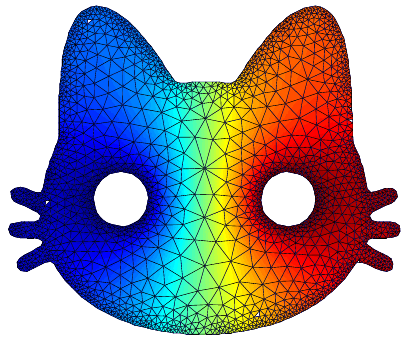
\includegraphics[scale=0.225]{cat.png}
				\end{figure}
			\end{column}
			\begin{column}{.1\textwidth}
				\centering
				$\large\rightarrow$
			\end{column}
			\begin{column}{.4\textwidth}
				\begin{figure}
					\raggedright
					\movie[autostart, showcontrols=true, width=.4\textwidth, externalviewer]{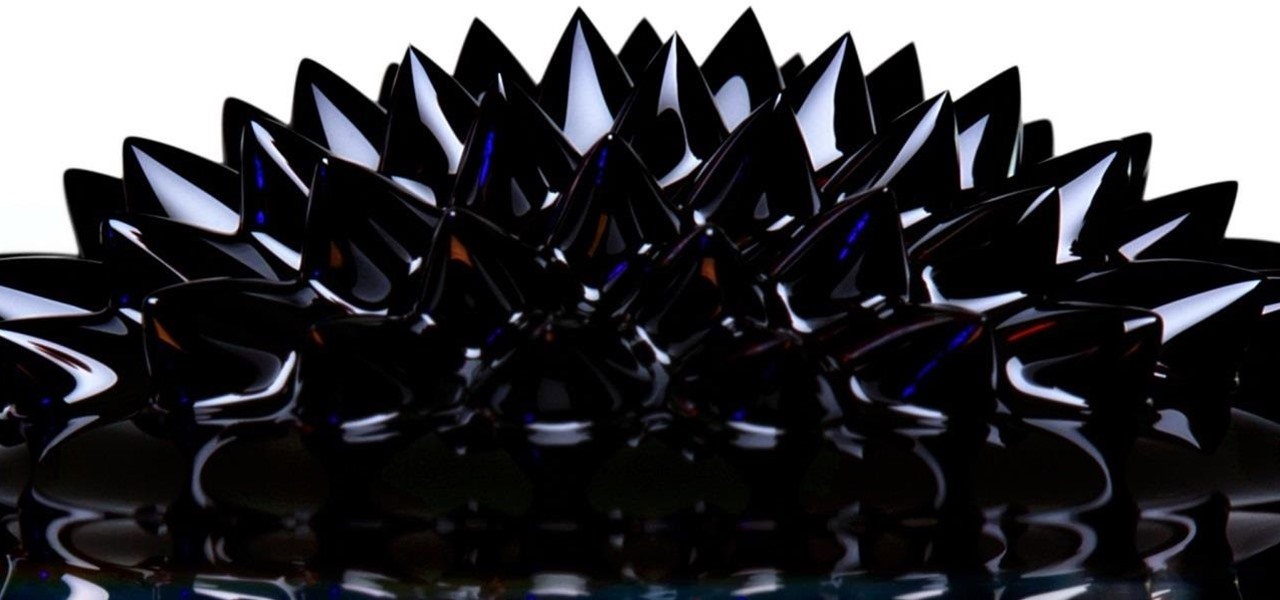
\includegraphics[scale=.11]{ferro2.jpg}}{ferro.gif}
				\end{figure}
			\end{column}
		\end{columns}
	
		\item Begin learning about ferrohydrodynamics. There is potential for this topic to be a large portion of my thesis.
		
		\item Advance the scientific understanding of ferrohydrodynamics though my computations.
	\end{itemize}

\end{frame}

\section{References}
\begin{frame}
	\textbf{References:}
	\begin{itemize}
		\item https://commons.wikimedia.org/wiki/File:North\_Carolina\_State\_University\_
		Athletic\_logo.svg
		
		\item http://asastudentcouncil.org/wp-content/uploads/2017/12/JHU-APL-Logo.png
		
		\item https://www.nvidia.com/content/dam/en-zz/es\_em/Solutions/Data-Center/tesla-v100/data-center-tesla-v100-pcie-625-ud@2x.jpg
		
		\item Maria Cameron. \textit{Elliptic}, Course Notes, 2018.
		
		\item https://img.wonderhowto.com/img/82/88/63513385636549/0/make-ferrofluid-liquid-future.1280x600.jpg
		
		\item https://www.reddit.com/r/gifs/comments/1ki7ea/ferrofluid\_sculpture/
	\end{itemize}
\end{frame}
\end{document}
